\documentclass{standalone}
\usepackage{tikz}
\usetikzlibrary{patterns, positioning}
\usepackage[sfdefault]{ClearSans} %% option 'sfdefault' activates Clear Sans as the default text font
\usepackage[T1]{fontenc}

\begin{document}
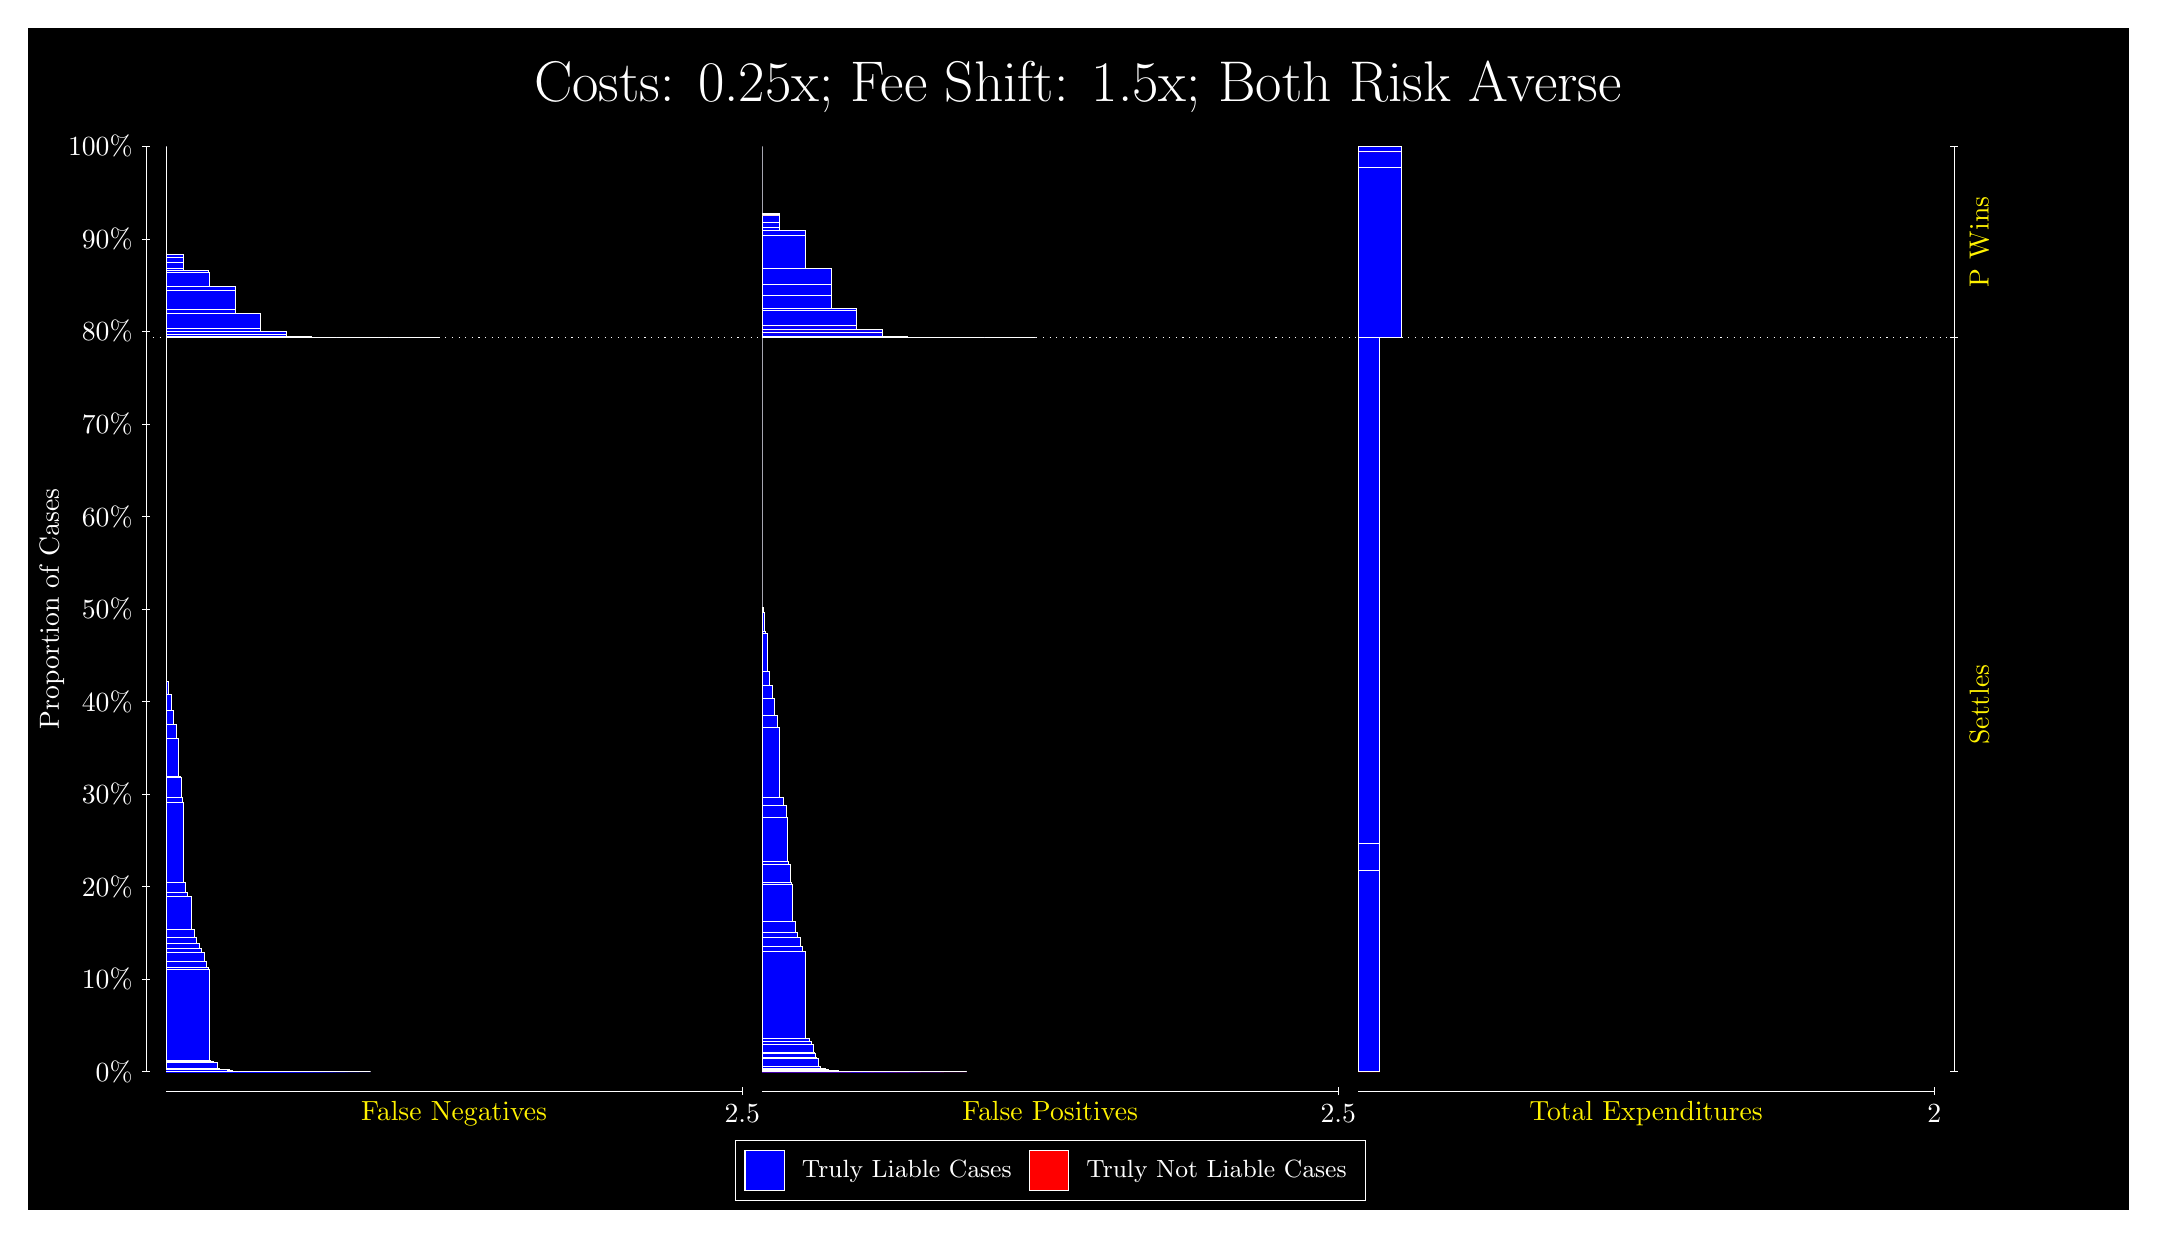
\begin{tikzpicture}
\draw[fill=black] (0,0) rectangle (26.667,15);
\draw[text=white] (0,13.5) rectangle (26.667,15) node[midway] {\huge Costs: 0.25x; Fee Shift: 1.5x; Both Risk Averse};
\draw[white, very thin] (1.5,1.75) -- (1.5,13.5);
\node[rotate=90, text=white, anchor=center] at (0.3, 7.625) {Proportion of Cases};
\draw[white, very thin] (1.45,1.75) -- (1.55,1.75);
\node[text=white, anchor=east] at (1.45, 1.75) {0\%};
\draw[white, very thin] (1.45,2.925) -- (1.55,2.925);
\node[text=white, anchor=east] at (1.45, 2.925) {10\%};
\draw[white, very thin] (1.45,4.1) -- (1.55,4.1);
\node[text=white, anchor=east] at (1.45, 4.1) {20\%};
\draw[white, very thin] (1.45,5.275) -- (1.55,5.275);
\node[text=white, anchor=east] at (1.45, 5.275) {30\%};
\draw[white, very thin] (1.45,6.45) -- (1.55,6.45);
\node[text=white, anchor=east] at (1.45, 6.45) {40\%};
\draw[white, very thin] (1.45,7.625) -- (1.55,7.625);
\node[text=white, anchor=east] at (1.45, 7.625) {50\%};
\draw[white, very thin] (1.45,8.8) -- (1.55,8.8);
\node[text=white, anchor=east] at (1.45, 8.8) {60\%};
\draw[white, very thin] (1.45,9.975) -- (1.55,9.975);
\node[text=white, anchor=east] at (1.45, 9.975) {70\%};
\draw[white, very thin] (1.45,11.15) -- (1.55,11.15);
\node[text=white, anchor=east] at (1.45, 11.15) {80\%};
\draw[white, very thin] (1.45,12.325) -- (1.55,12.325);
\node[text=white, anchor=east] at (1.45, 12.325) {90\%};
\draw[white, very thin] (1.45,13.5) -- (1.55,13.5);
\node[text=white, anchor=east] at (1.45, 13.5) {100\%};

\draw[white, very thin] (24.457,1.75) -- (24.457,13.5);
\draw[white, very thin] (24.407,1.75) -- (24.507,1.75);
\node[anchor=west] at (24.407, 1.75) {};
\draw[white, very thin] (24.407,11.073) -- (24.507,11.073);
\node[anchor=west] at (24.407, 11.073) {};
\draw[white, very thin] (24.407,13.5) -- (24.507,13.5);
\node[anchor=west] at (24.407, 13.5) {};

\draw[white, very thin, fill=blue] (1.75,1.75) rectangle (4.3482,1.75);
\draw[white, very thin, fill=blue] (1.75,1.75) rectangle (4.2018,1.75);
\draw[white, very thin, fill=blue] (1.75,1.75) rectangle (4.0554,1.75);
\draw[white, very thin, fill=blue] (1.75,1.75) rectangle (4.0229,1.75);
\draw[white, very thin, fill=blue] (1.75,1.75) rectangle (3.9091,1.75);
\draw[white, very thin, fill=blue] (1.75,1.75) rectangle (3.8765,1.75);
\draw[white, very thin, fill=blue] (1.75,1.75) rectangle (3.7627,1.75);
\draw[white, very thin, fill=blue] (1.75,1.75) rectangle (3.7302,1.75);
\draw[white, very thin, fill=blue] (1.75,1.75) rectangle (3.6976,1.75);
\draw[white, very thin, fill=blue] (1.75,1.75) rectangle (3.6163,1.75);
\draw[white, very thin, fill=blue] (1.75,1.75) rectangle (3.5838,1.75);
\draw[white, very thin, fill=blue] (1.75,1.75) rectangle (3.5513,1.75);
\draw[white, very thin, fill=blue] (1.75,1.75) rectangle (3.4699,1.75);
\draw[white, very thin, fill=blue] (1.75,1.75) rectangle (3.4374,1.75);
\draw[white, very thin, fill=blue] (1.75,1.75) rectangle (3.4049,1.75);
\draw[white, very thin, fill=blue] (1.75,1.75) rectangle (3.3723,1.75);
\draw[white, very thin, fill=blue] (1.75,1.75) rectangle (3.3236,1.75);
\draw[white, very thin, fill=blue] (1.75,1.75) rectangle (3.291,1.75);
\draw[white, very thin, fill=blue] (1.75,1.75) rectangle (3.2585,1.75);
\draw[white, very thin, fill=blue] (1.75,1.75) rectangle (3.226,1.75);
\draw[white, very thin, fill=blue] (1.75,1.75) rectangle (3.1772,1.75);
\draw[white, very thin, fill=blue] (1.75,1.75) rectangle (3.1447,1.75);
\draw[white, very thin, fill=blue] (1.75,1.75) rectangle (3.1121,1.75);
\draw[white, very thin, fill=blue] (1.75,1.75) rectangle (3.0796,1.75);
\draw[white, very thin, fill=blue] (1.75,1.75) rectangle (3.0471,1.75);
\draw[white, very thin, fill=blue] (1.75,1.75) rectangle (3.0308,1.75);
\draw[white, very thin, fill=blue] (1.75,1.75) rectangle (2.9983,1.75);
\draw[white, very thin, fill=blue] (1.75,1.75) rectangle (2.9657,1.75);
\draw[white, very thin, fill=blue] (1.75,1.75) rectangle (2.9332,1.75);
\draw[white, very thin, fill=blue] (1.75,1.75) rectangle (2.9007,1.75);
\draw[white, very thin, fill=blue] (1.75,1.75) rectangle (2.8844,1.7501);
\draw[white, very thin, fill=blue] (1.75,1.7501) rectangle (2.8519,1.7502);
\draw[white, very thin, fill=blue] (1.75,1.7502) rectangle (2.8194,1.7502);
\draw[white, very thin, fill=blue] (1.75,1.7502) rectangle (2.7868,1.7503);
\draw[white, very thin, fill=blue] (1.75,1.7503) rectangle (2.7543,1.7505);
\draw[white, very thin, fill=blue] (1.75,1.7505) rectangle (2.7218,1.7538);
\draw[white, very thin, fill=blue] (1.75,1.7538) rectangle (2.7055,1.7538);
\draw[white, very thin, fill=blue] (1.75,1.7538) rectangle (2.673,1.7538);
\draw[white, very thin, fill=blue] (1.75,1.7538) rectangle (2.6405,1.7544);
\draw[white, very thin, fill=blue] (1.75,1.7544) rectangle (2.6079,1.7555);
\draw[white, very thin, fill=blue] (1.75,1.7555) rectangle (2.5917,1.766);
\draw[white, very thin, fill=blue] (1.75,1.766) rectangle (2.5754,1.7663);
\draw[white, very thin, fill=blue] (1.75,1.7663) rectangle (2.5591,1.7725);
\draw[white, very thin, fill=blue] (1.75,1.7725) rectangle (2.5266,1.7747);
\draw[white, very thin, fill=blue] (1.75,1.7747) rectangle (2.4941,1.779);
\draw[white, very thin, fill=blue] (1.75,1.779) rectangle (2.4616,1.7835);
\draw[white, very thin, fill=blue] (1.75,1.7835) rectangle (2.429,1.7962);
\draw[white, very thin, fill=blue] (1.75,1.7962) rectangle (2.3965,1.8702);
\draw[white, very thin, fill=blue] (1.75,1.8702) rectangle (2.3802,1.8704);
\draw[white, very thin, fill=blue] (1.75,1.8704) rectangle (2.3477,1.8749);
\draw[white, very thin, fill=blue] (1.75,1.8749) rectangle (2.3152,1.8957);
\draw[white, very thin, fill=blue] (1.75,1.8957) rectangle (2.2989,3.0497);
\draw[white, very thin, fill=blue] (1.75,3.0497) rectangle (2.2827,3.0699);
\draw[white, very thin, fill=blue] (1.75,3.0699) rectangle (2.2664,3.1477);
\draw[white, very thin, fill=blue] (1.75,3.1477) rectangle (2.2501,3.1536);
\draw[white, very thin, fill=blue] (1.75,3.1536) rectangle (2.2339,3.2672);
\draw[white, very thin, fill=blue] (1.75,3.2672) rectangle (2.2013,3.3117);
\draw[white, very thin, fill=blue] (1.75,3.3117) rectangle (2.1688,3.3804);
\draw[white, very thin, fill=blue] (1.75,3.3804) rectangle (2.1363,3.4553);
\draw[white, very thin, fill=blue] (1.75,3.4553) rectangle (2.1037,3.5546);
\draw[white, very thin, fill=blue] (1.75,3.5546) rectangle (2.0712,3.9764);
\draw[white, very thin, fill=blue] (1.75,3.9764) rectangle (2.055,3.9786);
\draw[white, very thin, fill=blue] (1.75,3.9786) rectangle (2.0224,4.025);
\draw[white, very thin, fill=blue] (1.75,4.025) rectangle (1.9899,4.1596);
\draw[white, very thin, fill=blue] (1.75,4.1596) rectangle (1.9736,5.1724);
\draw[white, very thin, fill=blue] (1.75,5.1724) rectangle (1.9574,5.235);
\draw[white, very thin, fill=blue] (1.75,5.235) rectangle (1.9411,5.4815);
\draw[white, very thin, fill=blue] (1.75,5.4815) rectangle (1.9248,5.5051);
\draw[white, very thin, fill=blue] (1.75,5.5051) rectangle (1.9086,5.9857);
\draw[white, very thin, fill=blue] (1.75,5.9857) rectangle (1.876,6.1632);
\draw[white, very thin, fill=blue] (1.75,6.1632) rectangle (1.8435,6.3355);
\draw[white, very thin, fill=blue] (1.75,6.3355) rectangle (1.811,6.5473);
\draw[white, very thin, fill=blue] (1.75,6.5473) rectangle (1.7785,6.7044);
\draw[white, very thin, fill=red] (1.75,6.7044) rectangle (1.75,6.7044);
\draw[white, very thin, fill=blue] (1.75,6.7044) rectangle (1.75,11.073);
\draw[white, very thin, fill=blue] (1.75,11.073) rectangle (5.2265,11.073);
\draw[white, very thin, fill=blue] (1.75,11.073) rectangle (4.9012,11.073);
\draw[white, very thin, fill=blue] (1.75,11.073) rectangle (4.5759,11.073);
\draw[white, very thin, fill=blue] (1.75,11.073) rectangle (4.5759,11.073);
\draw[white, very thin, fill=blue] (1.75,11.073) rectangle (4.2506,11.073);
\draw[white, very thin, fill=blue] (1.75,11.073) rectangle (4.2506,11.073);
\draw[white, very thin, fill=blue] (1.75,11.073) rectangle (3.9253,11.074);
\draw[white, very thin, fill=blue] (1.75,11.074) rectangle (3.9172,11.074);
\draw[white, very thin, fill=blue] (1.75,11.074) rectangle (3.6,11.086);
\draw[white, very thin, fill=blue] (1.75,11.086) rectangle (3.5919,11.086);
\draw[white, very thin, fill=blue] (1.75,11.086) rectangle (3.2748,11.108);
\draw[white, very thin, fill=blue] (1.75,11.108) rectangle (3.2748,11.155);
\draw[white, very thin, fill=blue] (1.75,11.155) rectangle (3.2666,11.155);
\draw[white, very thin, fill=blue] (1.75,11.155) rectangle (3.2666,11.155);
\draw[white, very thin, fill=blue] (1.75,11.155) rectangle (2.9495,11.19);
\draw[white, very thin, fill=blue] (1.75,11.19) rectangle (2.9495,11.384);
\draw[white, very thin, fill=blue] (1.75,11.384) rectangle (2.9413,11.384);
\draw[white, very thin, fill=blue] (1.75,11.384) rectangle (2.9413,11.384);
\draw[white, very thin, fill=blue] (1.75,11.384) rectangle (2.6242,11.436);
\draw[white, very thin, fill=blue] (1.75,11.436) rectangle (2.6242,11.675);
\draw[white, very thin, fill=blue] (1.75,11.675) rectangle (2.6242,11.724);
\draw[white, very thin, fill=blue] (1.75,11.724) rectangle (2.6161,11.724);
\draw[white, very thin, fill=blue] (1.75,11.724) rectangle (2.6161,11.724);
\draw[white, very thin, fill=blue] (1.75,11.724) rectangle (2.6161,11.725);
\draw[white, very thin, fill=blue] (1.75,11.725) rectangle (2.2989,11.902);
\draw[white, very thin, fill=blue] (1.75,11.902) rectangle (2.2908,11.903);
\draw[white, very thin, fill=blue] (1.75,11.903) rectangle (2.2908,11.925);
\draw[white, very thin, fill=blue] (1.75,11.925) rectangle (1.9736,11.95);
\draw[white, very thin, fill=blue] (1.75,11.95) rectangle (1.9736,11.951);
\draw[white, very thin, fill=blue] (1.75,11.951) rectangle (1.9655,12.026);
\draw[white, very thin, fill=blue] (1.75,12.026) rectangle (1.9655,12.097);
\draw[white, very thin, fill=blue] (1.75,12.097) rectangle (1.9655,12.133);
\draw[white, very thin, fill=red] (1.75,12.133) rectangle (1.75,12.133);
\draw[white, very thin, fill=blue] (1.75,12.133) rectangle (1.75,13.5);
\draw[white, very thin, fill=red] (9.3189,1.75) rectangle (11.917,1.75);
\draw[white, very thin, fill=blue] (9.3189,1.75) rectangle (11.917,1.75);
\draw[white, very thin, fill=red] (9.3189,1.75) rectangle (11.624,1.75);
\draw[white, very thin, fill=blue] (9.3189,1.75) rectangle (11.624,1.75);
\draw[white, very thin, fill=blue] (9.3189,1.75) rectangle (11.592,1.75);
\draw[white, very thin, fill=red] (9.3189,1.75) rectangle (11.332,1.75);
\draw[white, very thin, fill=blue] (9.3189,1.75) rectangle (11.332,1.75);
\draw[white, very thin, fill=blue] (9.3189,1.75) rectangle (11.299,1.75);
\draw[white, very thin, fill=blue] (9.3189,1.75) rectangle (11.266,1.75);
\draw[white, very thin, fill=red] (9.3189,1.75) rectangle (11.185,1.75);
\draw[white, very thin, fill=blue] (9.3189,1.75) rectangle (11.185,1.75);
\draw[white, very thin, fill=red] (9.3189,1.75) rectangle (11.039,1.75);
\draw[white, very thin, fill=blue] (9.3189,1.75) rectangle (11.039,1.75);
\draw[white, very thin, fill=blue] (9.3189,1.75) rectangle (11.006,1.75);
\draw[white, very thin, fill=blue] (9.3189,1.75) rectangle (10.974,1.75);
\draw[white, very thin, fill=blue] (9.3189,1.75) rectangle (10.941,1.75);
\draw[white, very thin, fill=red] (9.3189,1.75) rectangle (10.892,1.75);
\draw[white, very thin, fill=blue] (9.3189,1.75) rectangle (10.892,1.75);
\draw[white, very thin, fill=blue] (9.3189,1.75) rectangle (10.86,1.75);
\draw[white, very thin, fill=red] (9.3189,1.75) rectangle (10.746,1.75);
\draw[white, very thin, fill=blue] (9.3189,1.75) rectangle (10.746,1.75);
\draw[white, very thin, fill=blue] (9.3189,1.75) rectangle (10.714,1.75);
\draw[white, very thin, fill=blue] (9.3189,1.75) rectangle (10.681,1.75);
\draw[white, very thin, fill=blue] (9.3189,1.75) rectangle (10.648,1.7501);
\draw[white, very thin, fill=blue] (9.3189,1.7501) rectangle (10.616,1.7501);
\draw[white, very thin, fill=red] (9.3189,1.7501) rectangle (10.6,1.7501);
\draw[white, very thin, fill=blue] (9.3189,1.7501) rectangle (10.6,1.7501);
\draw[white, very thin, fill=blue] (9.3189,1.7501) rectangle (10.567,1.7502);
\draw[white, very thin, fill=blue] (9.3189,1.7502) rectangle (10.535,1.7502);
\draw[white, very thin, fill=red] (9.3189,1.7502) rectangle (10.453,1.7502);
\draw[white, very thin, fill=blue] (9.3189,1.7502) rectangle (10.453,1.7506);
\draw[white, very thin, fill=blue] (9.3189,1.7506) rectangle (10.421,1.7506);
\draw[white, very thin, fill=blue] (9.3189,1.7506) rectangle (10.388,1.7511);
\draw[white, very thin, fill=blue] (9.3189,1.7511) rectangle (10.356,1.7564);
\draw[white, very thin, fill=blue] (9.3189,1.7564) rectangle (10.323,1.7586);
\draw[white, very thin, fill=red] (9.3189,1.7586) rectangle (10.307,1.7586);
\draw[white, very thin, fill=blue] (9.3189,1.7586) rectangle (10.307,1.7589);
\draw[white, very thin, fill=blue] (9.3189,1.7589) rectangle (10.291,1.7642);
\draw[white, very thin, fill=blue] (9.3189,1.7642) rectangle (10.274,1.7656);
\draw[white, very thin, fill=blue] (9.3189,1.7656) rectangle (10.242,1.7684);
\draw[white, very thin, fill=blue] (9.3189,1.7684) rectangle (10.209,1.7686);
\draw[white, very thin, fill=red] (9.3189,1.7686) rectangle (10.161,1.7686);
\draw[white, very thin, fill=blue] (9.3189,1.7686) rectangle (10.161,1.7783);
\draw[white, very thin, fill=blue] (9.3189,1.7783) rectangle (10.128,1.7904);
\draw[white, very thin, fill=blue] (9.3189,1.7904) rectangle (10.095,1.7948);
\draw[white, very thin, fill=blue] (9.3189,1.7948) rectangle (10.063,1.8137);
\draw[white, very thin, fill=blue] (9.3189,1.8137) rectangle (10.03,1.9239);
\draw[white, very thin, fill=red] (9.3189,1.9239) rectangle (10.014,1.9239);
\draw[white, very thin, fill=blue] (9.3189,1.9239) rectangle (10.014,1.9333);
\draw[white, very thin, fill=blue] (9.3189,1.9333) rectangle (9.9979,1.9823);
\draw[white, very thin, fill=blue] (9.3189,1.9823) rectangle (9.9816,1.9886);
\draw[white, very thin, fill=blue] (9.3189,1.9886) rectangle (9.9654,2.1003);
\draw[white, very thin, fill=blue] (9.3189,2.1003) rectangle (9.9491,2.1318);
\draw[white, very thin, fill=blue] (9.3189,2.1318) rectangle (9.9166,2.1687);
\draw[white, very thin, fill=blue] (9.3189,2.1687) rectangle (9.884,2.1706);
\draw[white, very thin, fill=red] (9.3189,2.1706) rectangle (9.8678,2.1706);
\draw[white, very thin, fill=blue] (9.3189,2.1706) rectangle (9.8678,3.2782);
\draw[white, very thin, fill=blue] (9.3189,3.2782) rectangle (9.8353,3.3419);
\draw[white, very thin, fill=blue] (9.3189,3.3419) rectangle (9.8027,3.4514);
\draw[white, very thin, fill=blue] (9.3189,3.4514) rectangle (9.7702,3.5201);
\draw[white, very thin, fill=blue] (9.3189,3.5201) rectangle (9.7377,3.6561);
\draw[white, very thin, fill=blue] (9.3189,3.6561) rectangle (9.7051,4.1335);
\draw[white, very thin, fill=blue] (9.3189,4.1335) rectangle (9.6889,4.1576);
\draw[white, very thin, fill=blue] (9.3189,4.1576) rectangle (9.6726,4.384);
\draw[white, very thin, fill=blue] (9.3189,4.384) rectangle (9.6563,4.4234);
\draw[white, very thin, fill=blue] (9.3189,4.4234) rectangle (9.6401,4.982);
\draw[white, very thin, fill=blue] (9.3189,4.982) rectangle (9.6238,5.133);
\draw[white, very thin, fill=blue] (9.3189,5.133) rectangle (9.5913,5.2271);
\draw[white, very thin, fill=blue] (9.3189,5.2271) rectangle (9.5588,5.232);
\draw[white, very thin, fill=blue] (9.3189,5.232) rectangle (9.5425,6.1182);
\draw[white, very thin, fill=blue] (9.3189,6.1182) rectangle (9.51,6.2753);
\draw[white, very thin, fill=blue] (9.3189,6.2753) rectangle (9.4774,6.4871);
\draw[white, very thin, fill=blue] (9.3189,6.4871) rectangle (9.4449,6.6594);
\draw[white, very thin, fill=blue] (9.3189,6.6594) rectangle (9.4124,6.8369);
\draw[white, very thin, fill=blue] (9.3189,6.8369) rectangle (9.3799,7.3175);
\draw[white, very thin, fill=blue] (9.3189,7.3175) rectangle (9.3636,7.3411);
\draw[white, very thin, fill=blue] (9.3189,7.3411) rectangle (9.3473,7.5876);
\draw[white, very thin, fill=blue] (9.3189,7.5876) rectangle (9.3311,7.6502);
\draw[white, very thin, fill=blue] (9.3189,7.6502) rectangle (9.3189,11.073);
\draw[white, very thin, fill=red] (9.3189,11.073) rectangle (12.795,11.073);
\draw[white, very thin, fill=blue] (9.3189,11.073) rectangle (12.795,11.073);
\draw[white, very thin, fill=red] (9.3189,11.073) rectangle (12.47,11.073);
\draw[white, very thin, fill=blue] (9.3189,11.073) rectangle (12.47,11.073);
\draw[white, very thin, fill=red] (9.3189,11.073) rectangle (12.145,11.073);
\draw[white, very thin, fill=blue] (9.3189,11.073) rectangle (12.145,11.073);
\draw[white, very thin, fill=blue] (9.3189,11.073) rectangle (12.145,11.073);
\draw[white, very thin, fill=blue] (9.3189,11.073) rectangle (11.819,11.073);
\draw[white, very thin, fill=red] (9.3189,11.073) rectangle (11.819,11.073);
\draw[white, very thin, fill=blue] (9.3189,11.073) rectangle (11.819,11.073);
\draw[white, very thin, fill=red] (9.3189,11.073) rectangle (11.494,11.073);
\draw[white, very thin, fill=blue] (9.3189,11.073) rectangle (11.494,11.075);
\draw[white, very thin, fill=red] (9.3189,11.075) rectangle (11.169,11.075);
\draw[white, very thin, fill=blue] (9.3189,11.075) rectangle (11.169,11.09);
\draw[white, very thin, fill=blue] (9.3189,11.09) rectangle (10.844,11.133);
\draw[white, very thin, fill=red] (9.3189,11.133) rectangle (10.844,11.133);
\draw[white, very thin, fill=blue] (9.3189,11.133) rectangle (10.844,11.173);
\draw[white, very thin, fill=red] (9.3189,11.173) rectangle (10.835,11.173);
\draw[white, very thin, fill=blue] (9.3189,11.173) rectangle (10.835,11.173);
\draw[white, very thin, fill=blue] (9.3189,11.173) rectangle (10.518,11.222);
\draw[white, very thin, fill=red] (9.3189,11.222) rectangle (10.518,11.222);
\draw[white, very thin, fill=blue] (9.3189,11.222) rectangle (10.518,11.42);
\draw[white, very thin, fill=blue] (9.3189,11.42) rectangle (10.518,11.444);
\draw[white, very thin, fill=blue] (9.3189,11.444) rectangle (10.51,11.444);
\draw[white, very thin, fill=red] (9.3189,11.444) rectangle (10.51,11.444);
\draw[white, very thin, fill=blue] (9.3189,11.444) rectangle (10.51,11.444);
\draw[white, very thin, fill=blue] (9.3189,11.444) rectangle (10.193,11.614);
\draw[white, very thin, fill=blue] (9.3189,11.614) rectangle (10.193,11.747);
\draw[white, very thin, fill=blue] (9.3189,11.747) rectangle (10.193,11.952);
\draw[white, very thin, fill=blue] (9.3189,11.952) rectangle (10.185,11.952);
\draw[white, very thin, fill=red] (9.3189,11.952) rectangle (10.185,11.952);
\draw[white, very thin, fill=blue] (9.3189,11.952) rectangle (10.185,11.952);
\draw[white, very thin, fill=blue] (9.3189,11.952) rectangle (9.8678,12.365);
\draw[white, very thin, fill=blue] (9.3189,12.365) rectangle (9.8678,12.44);
\draw[white, very thin, fill=blue] (9.3189,12.44) rectangle (9.8597,12.44);
\draw[white, very thin, fill=red] (9.3189,12.44) rectangle (9.8597,12.44);
\draw[white, very thin, fill=blue] (9.3189,12.44) rectangle (9.8597,12.44);
\draw[white, very thin, fill=blue] (9.3189,12.44) rectangle (9.5425,12.475);
\draw[white, very thin, fill=blue] (9.3189,12.475) rectangle (9.5425,12.531);
\draw[white, very thin, fill=blue] (9.3189,12.531) rectangle (9.5425,12.622);
\draw[white, very thin, fill=blue] (9.3189,12.622) rectangle (9.5344,12.622);
\draw[white, very thin, fill=blue] (9.3189,12.622) rectangle (9.5344,12.632);
\draw[white, very thin, fill=red] (9.3189,12.632) rectangle (9.5344,12.632);
\draw[white, very thin, fill=blue] (9.3189,12.632) rectangle (9.5344,12.648);
\draw[white, very thin, fill=red] (9.3189,12.648) rectangle (9.3189,12.648);
\draw[white, very thin, fill=blue] (9.3189,12.648) rectangle (9.3189,13.5);
\draw[white, very thin, fill=red] (16.888,1.75) rectangle (17.162,1.75);
\draw[white, very thin, fill=blue] (16.888,1.75) rectangle (17.162,4.306);
\draw[white, very thin, fill=red] (16.888,4.306) rectangle (17.162,4.306);
\draw[white, very thin, fill=blue] (16.888,4.306) rectangle (17.162,4.6488);
\draw[white, very thin, fill=red] (16.888,4.6488) rectangle (17.162,4.6488);
\draw[white, very thin, fill=blue] (16.888,4.6488) rectangle (17.162,11.073);
\draw[white, very thin, fill=red] (16.888,11.073) rectangle (17.437,11.073);
\draw[white, very thin, fill=blue] (16.888,11.073) rectangle (17.437,13.233);
\draw[white, very thin, fill=red] (16.888,13.233) rectangle (17.437,13.233);
\draw[white, very thin, fill=blue] (16.888,13.233) rectangle (17.437,13.432);
\draw[white, very thin, fill=red] (16.888,13.432) rectangle (17.437,13.432);
\draw[white, very thin, fill=blue] (16.888,13.432) rectangle (17.437,13.5);
\draw[white, dotted] (1.5,11.073) -- (24.457,11.073);
\draw[white, very thin] (1.75,1.5) -- (9.0689,1.5);
\node[text=yellow, anchor=north] at (5.4094, 1.5) {False Negatives};
\draw[white, very thin] (9.0689,1.45) -- (9.0689,1.55);
\node[text=white, anchor=north] at (9.0689, 1.45) {2.5};

\draw[white, very thin] (9.3189,1.5) -- (16.638,1.5);
\node[text=yellow, anchor=north] at (12.978, 1.5) {False Positives};
\draw[white, very thin] (16.638,1.45) -- (16.638,1.55);
\node[text=white, anchor=north] at (16.638, 1.45) {2.5};

\draw[white, very thin] (16.888,1.5) -- (24.207,1.5);
\node[text=yellow, anchor=north] at (20.547, 1.5) {Total Expenditures};
\draw[white, very thin] (24.207,1.45) -- (24.207,1.55);
\node[text=white, anchor=north] at (24.207, 1.45) {2};

\node[text=yellow, centered, rotate=90] at (24.777, 6.4113) {Settles};
\node[text=yellow, centered, rotate=90] at (24.777, 12.286) {P Wins};

\draw (12.978300999999998,1.5) node[draw=none] (baseCoordinate) {};
\begin{scope}[align=center]
        \matrix[scale=0.5, draw=white, below=0.5cm of baseCoordinate, nodes={draw}, column sep=0.1cm]{
            \node[rectangle, draw, minimum width=0.5cm, minimum height=0.5cm, fill=blue] {}; &
            \node[draw=none, font=\small, text=white] (B) {Truly Liable Cases}; &
            \node[rectangle, draw, minimum width=0.5cm, minimum height=0.5cm, fill=red] {}; &
            \node[draw=none, font=\small, text=white] (B) {Truly Not Liable Cases}; \\
            };
\end{scope}

\end{tikzpicture}
\end{document}